\documentclass[a4paper]{article}
\usepackage[brazilian]{babel}
\usepackage{subfig}
\usepackage{booktabs}
\usepackage{graphicx}
%-----------------------------------------------------------------
\title{MS 680 - Modelos matem\'{a}ticos aplicados a Biologia}
\author{122830 Alcides Goldoni Junior\\
  \Small Primeira prova \\
}%Fechando Title
\begin{document}
\maketitle
%----------------------------------------------------------------
%Seções
%----------------------------------------------------------------
\newpage
\begin{enumerate}
%Questao 1-------------------------------------------------------
\item
Vamos modelar a polui\c{c}\~ao de um rio seguindo as seguintes premissas: um rio dividido em sete setores longitudinais um seguido do outro; fluxo de \'agua limpa entrando por afluentes e saindo por atividades agr\'icolas j\'a polu\'ida, fazendo dessa forma um fluxo diferente para cada setor do rio, por\'em com um volume constante (o volume de \'agua que entra no primeiro setor do rio \'e igual ao volume de \'agua que sai no \'ultimo setor); polui\c{c}\~ao inicial diferente para cada setor; valor de decaimento de polui\c{c}\~ao diferente para cada setor; descarte de poluente diferente em cada setor.
\\
O sistema que melhor modela essa situa\c{c}\~ao \'e:
\begin{equation}
\frac{dP}{dt} = P\textsubscript{is} + \frac{P\textsubscript{s\_ant}F }{V} - PD - PA + Q + R
\end{equation}
onde:
\begin{itemize}
\item$P\textsubscript{is}$ \'e a polui\c{c}\~ao inicial do setor;
\item$P\textsubscript{s\_ant}$ \'e a quantidade de polui\c{c}\~ao vindo do setor anterior;
\item$F$ \'e o fluxo de \'agua vindo do setor anterior;
\item$V$ \'e o volume de \'agua;
\item$P$ \'e a polui\c{c}\~ao atual do setor;
\item$D$ \'e o decaimento da polui\c{c}\~ao daquele setor;
\item$A$ \'e a atividade agricola do setor;
\item$Q$ \'e a fonte de poluente do setor e
\item$R$ \'e a quantidade de \'agua limpa de afluentes.
\end{itemize}
\\
Para o caso do primeiro setor, a polui\c{c}\~ao que vem do setor anterior \'e zero e n\~ao \'e colocada na simula\c{c}\~ao.
\\
Para a simula\c{c}\~ao foram usados n\'umeros aleat\'orios, apenas para obter a visualiza\c{c}\~ao do que poderia ocorrer. Para diferentes ordens de grandeza de fluxo e fonte, obtemos resultados bem diferentes. A simula\c{c}\~ao foi escrita em Python.
\\
\begin{table}[h!]
\centering
\caption{Valores da simula\c{c}\~ao da polui\c{c}\~ao da represa por setor}
\begin{tabular}{|c|c|c|c|c|c|c|}
\hline
Setor &Fluxo 	& 	Afluente & Atividade Agr\'icola& Decaimento & Fonte & Polui\c{c}\~ao Inicial\\
\hline
1&0.9 	&	0.3	&	0.31		&	0.05	&	0.5	&	5.0	\\
2&0.45	&	0.4	&	0		&	0.06	&	0.6	&	2.7	\\
3&0.95	&	0.31	&	0.33		&	0.1	&	0.2	&	3.1	\\
4&0.6 	&	0.21	&	0.18		&	0.08	&	0.9	&	3.6	\\
5&0.87	&	0.27	&	0.11		&	0.09	&	0.3	&	3.0	\\
6&0.39	&	0.19	&	0		&	0.044	&	0.1	&	4.3	\\
7&0.77	&	0.2	&	0.27		&	0.03	&	0.9	&	9.3	\\
\hline
\end{tabular}
\end{table}

\begin{figure}[h]
\centering
\caption{Gr\'afico da concentra\c{c}\~ao do poluente por setor}
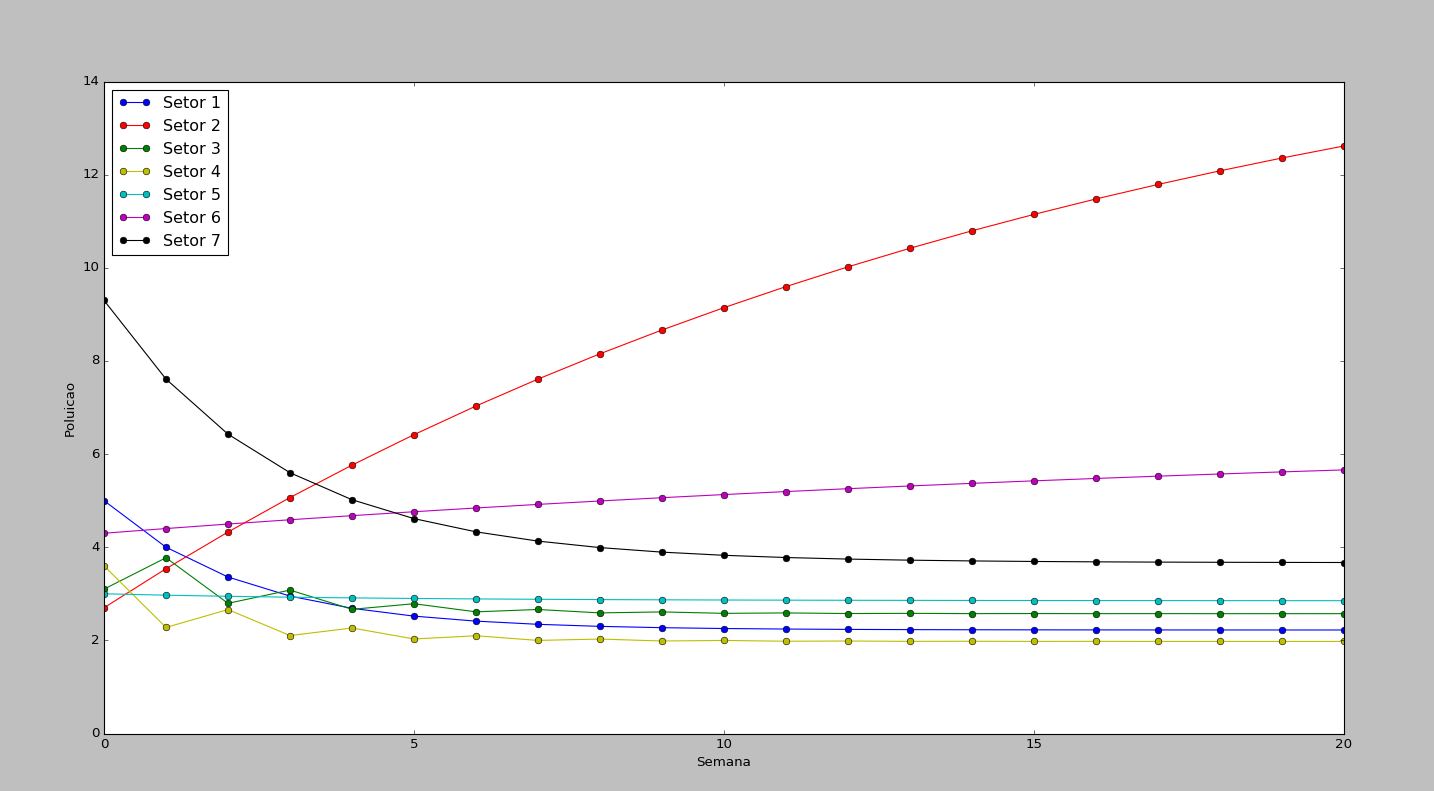
\includegraphics[scale=0.25]{simulacao1.png}
\end{figure}
\\
\begin{table}[h!]
\centering
\caption{Valores da simula\c{c}\~ao da polui\c{c}\~ao da represa por setor}
\begin{tabular}{|c|c|c|c|c|c|c|}
\hline
Setor &Fluxo 	& 	Afluente & Atividade Agr\'icola& Decaimento & Fonte & Polui\c{c}\~ao Inicial\\
\hline
1&0.09 	&	0.3	&	0.31		&	0.05	&	5	&	5.0	\\
2&0.045	&	0.4	&	0		&	0.06	&	6	&	2.7	\\
3&0.095	&	0.31	&	0.33		&	0.1	&	2	&	3.1	\\
4&0.06 	&	0.21	&	0.18		&	0.08	&	9	&	3.6	\\
5&0.087	&	0.27	&	0.11		&	0.09	&	3	&	3.0	\\
6&0.039	&	0.19	&	0		&	0.044	&	1	&	4.3	\\
7&0.077	&	0.2	&	0.27		&	0.03	&	9	&	9.3	\\
\hline
\end{tabular}
\end{table}

\begin{figure}[h]
\centering
\caption{Gr\'afico da concentra\c{c}\~ao do poluente por setor}
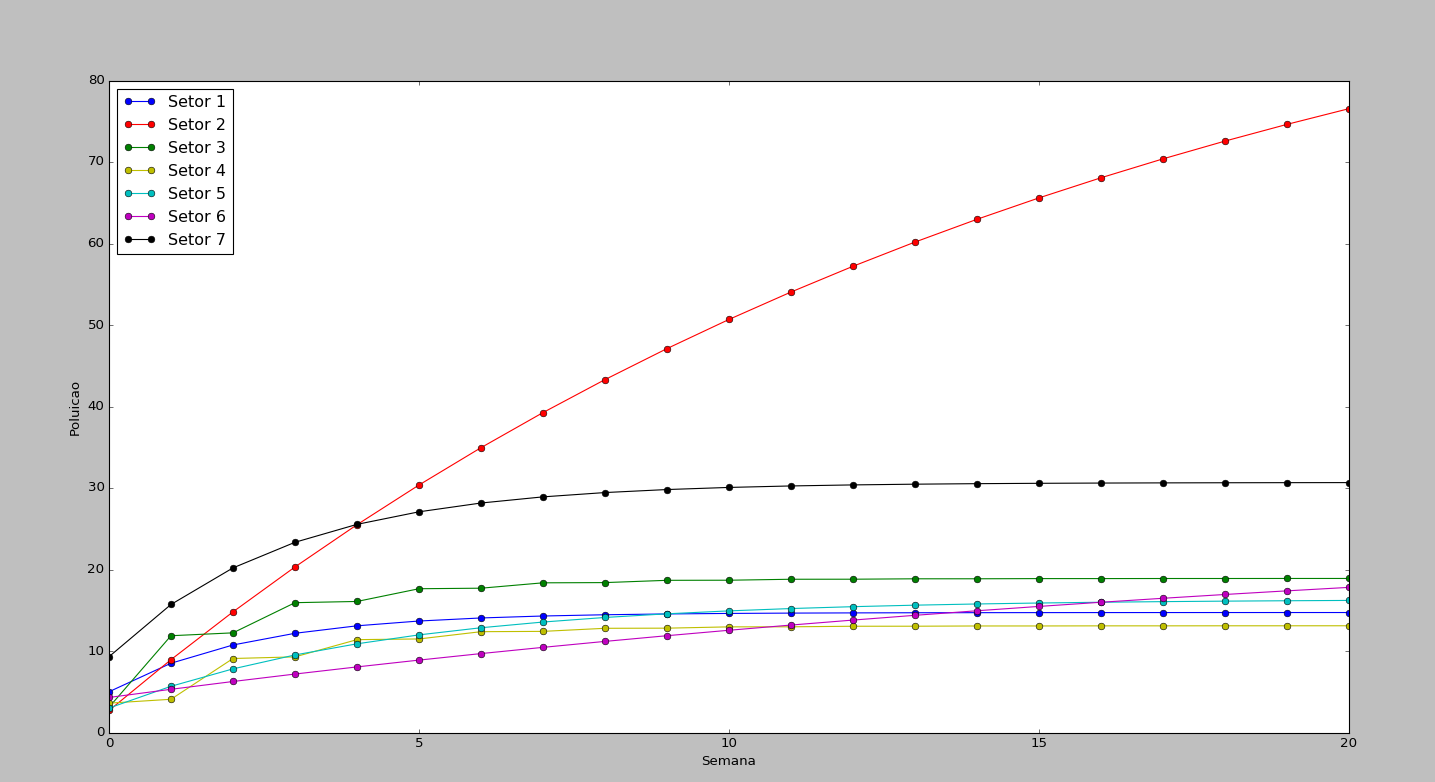
\includegraphics[scale=0.25]{simulacao2.png}
\end{figure}
\\
Mesmo com essas mudan\c{c}as, vemos que existe uma tend\^encia a estabilidade na maioria dos setores do rio.
\\
\'E poss\'ivel ver tamb\'em a influ\^encia da atividade agr\'icola, pois onde ela n\~ao existe, setores 2 e 6, a polui\c{c}\~ao tende a crescer.
\\
Outras simula\c{c}\~oes variando outros paramentros poderiam ser realizadas e dessa forma, obter diferentes gr\'aficos de diferentes situa\c{c}\~oes.
\\


%Questao 2-------------------------------------------------------
\item
Considerando a situa\c{c}\~ao de uma doen\c{c}a com caracter\'isticas parecidas com a gripe, onde o infectado se torna resistente ou removido e ainda existe vacina\c{c}\~ao, utilizando tamb\'em do modelo SIRS cont\'inuo para descrever o comportamento da doen\c{c}a, vamos levar em considera\c{c}\~ao que filhos de suscet\'ivel \'e suscet\'ivel, filho de infectado \'e infectado e filho de resistente \'e resistente. 
\\
Dessa forma, o sistema de equa\c{c}\~oes que melhor descreve essa situa\c{c}\~ao \'e:
\\
\begin{equation}
\left\{\begin{array}{l}
\frac{dS}{dt} = -\alpha SI + \lambda S + \phi R\\
\\
\frac{dS}{dt} = \alpha SI - \beta R - \gamma r + \varepsilon I\\
\\
\frac{dR}{dt} = \beta R + \omega R - \phi R \\
\\
\frac{dr}{dt} = \gamma r \\
\end{array}
\end{equation}
O modelo acima reflete o que acontece com a popula\c{c}\~ao quando ainda n\~ao se tem a vacina\c{c}\~ao, onde:
\begin{itemize}
\item$S$ s\~ao os indiv\'iduos suscet\'iveis;
\item$I$ s\~ao os indiv\'iduos infectados;
\item$R$ s\~ao os indiv\'iduos resistentes;
\item$r$ s\~ao os indiv\'iduos removidos;
\item$\alpha$ \'e a taxa de infec\c{c}\~ao de indiv\'iduos suscet\'iveis;
\item$\lambda$ \'e a taxa crescimento de indiv\'iduos suscet\'iveis;
\item$\beta$ \'e a taxa  de indiv\'iduosde infectados que se tornam resistentes;
\item$\varepsilon$ \'e a taxa crescimento de indiv\'iduos infectados;
\item$\gamma$ \'e a taxa  de indiv\'iduosde que s\~ao removidos;
\item$\omega$ \'e a taxa de crescimento de indiv\'iduos resistentes e
\item$\phi$ \'e a taxa de indiv\'iduos infectados se voltam a ser suscet\'iveis.
\end{itemize}
\\
Agora, vamos incluir a vacina\c{c}\~ao dos indiv\'iduos suscet\'iveis:
\\
\begin{equation}
\left\{\begin{array}{l}
\frac{dS}{dt} = -\alpha SI + \lambda S + \phi R - \mu S \\
\\
\frac{dI}{dt} = \alpha SI - \beta R - \gamma r + \varepsilon I\\
\\
\frac{dR}{dt} = \beta R + \omega R + \phi R + \mu S \\
\\
\frac{dr}{dt} = \gamma r \\
\end{array}
\end{equation}
\\
Com a vacina\c{c}\~ao, temos uma taxa $\mu$ de pessoas que eram suscet\'iveis e se tornam resistentes de forma direta. Dessa forma,
\\

%Questao 3-------------------------------------------------------
\item
De tudo o que vimos na disciplina, o fato que me deixou mais surpreso foi um exemplo, dado apenas como hist\'oria vivida pelo Prof. Joni, da constru\c{c}\~ao de uma represa, onde foram retirados v\'arios animais da \'area que seria alagada e recolocados em outro lugar.
\\
A atitude me parecia coerente, at\'e come\c{c}ar a estudar a Capacidade de Suporte, ap\'os isso, pude entender que ao inv\'es dos animais daquela regi\~ao morrerem devido ao alagamento, por terem sido removidos a um lugar que n\~ao seria alagado, eles acabaram morrendo de fome, afinal, o meio n\~ao estava preparado para manter todos aqueles animais.
\\
Com um estudo r\'apido, que qualquer aluno que tenha cursado essa disciplina poderia fazer, seria f\'acil mostrar que remover os animais de uma regi\~ao e levar pra outra deveria respeitar um conceito simples, por\'em muito importante, que \'e a capacidade de suporte do meio.
\\
%Questao 4-------------------------------------------------------
\item
Um outro problema em rela\c{c}\~ao a disciplina \'e que ela requer conhecimentos de equa\c{c}\~oes diferenciais ordin\'arias, ent\~ao, talvez fosse interessante que ela tivesse pr\'e requisito como C\'alculo 3 (MA 311). Na parte de simula\c{c}\~ao, seria interssante que o aluno tivesse conhecimento de algor\'itmos, dessa forma, seria interessante que j\'a tivesse feito Algor\'itmos e programa\c{c}\~ao de computadores (MC 102). Mas, como a parte de simula\c{c}\~ao n\~ao foi t\~ao exigida, apenas C\'alculo 3 j\'a seria interessamte. 
\\
%Questao 5-------------------------------------------------------
\item
De acordo com a ementa da disciplina, abordamos de forma muito boa os problemas de din\^amica populacional, incluindo competi\c{c}\~ao intra e interespec\'ifica, por meio das equa\c{c}\~oes recursivas e equa\c{c}\~oes diferenciais, tendo muitos exemplos em aula e nos dois projetos. 
\\
Os assuntos que gostaria de ter estudado com mais enf\^ase s\~ao os processos fisiol\'ogicos, principalmente aqueles relacionados a doen\c{c}as tais como a dengue nos seres humanos, a febre aftosa em gado, a podrid\~ao (vermelha, fusarium ou abacaxi) da cana-de-a\c{c}ucar e como isso afeta o organismo e/ou a sociedade.
\\
Outro t\'opico interessante seria o crescimento de tumores.
\\
A grande maioria dos exemplos dado em sala, foram relacionados a din\^amica populacional com ou sem competi\c{c}\~ao e decaimento de poluentes, mostrando como isso afeta popula\c{c}\~oes. Contudo, exemplos com doen\c{c}as foram abordados apenas no final do curso. Esse tipo de exemplo daria mais dinamismo a aula.
\\
%Questao 6-------------------------------------------------------
\item
As equ\c{c}\~oes de crescimento populacional podem ser adaptadas para as doen\c{c}as. Como citei na quest\~ao 5, vou levar em considera\c{c}\~ao o crescimento de um tumor.
\\
O material gen\'etico (DNA) de uma c\'elula pode sofrer altera\c{c}\~oes e desenvolver muta\c{c}\~oes que podem afetar o crescimento normal das estruturas celulares. Um mecanismo comumente afetado \'e o de divis\~ao das c\'elulas, fazendo com que elas se proliferem de maneira anormal. Essa prolifera\c{c}\~ao anormal provoca a forma\c{c}\~ao de massa celular, chamada de tumor.
\\
Para modelar esse problema de crescimento de massa de forma anormal, vou utilizar a equa\c{c}\~ao de Gopertz:
\\
\begin{equation}
\frac{dN}{dt} = r N ln (\frac{K}{N})
\end{equation}
Onde:
\\
$N(t)$ \'e a popula\c{c}\~ao das c\'elulas no instante t;
\\
$r$ \'e a taxa de crescimento das c\'elulas;
\\
$K$ \'e a capacidade de suporte, nesse caso, o tamanho m\'aximo que esse tumor pode atingir.
\\
%Consultando o trabalho de Jos\'e S\'ergio Domingues, IFNMG - Pirapora / MG de desenvolvimento de tumores, consultei os seguintes valores para os par\^ametros da Equa\c{c}\~ao de Gompertz:
%\\
%\begin{table}
%\centering
%\caption{Valores para a curva de Gompertz}
%\begin{tabular}{|c|c|c|}
%\hline
%r	&	K	&	N(0)\\
%\hline
%0,006	&	10e13	&	10e9\\
%\hline
%\end{tabular}
%\end{table}
Sabendo o valor inicial (popula\c{c}\~ao) das c\'elulas tumorais no instante $N(0)$ e sabendo a solu\c{c}\~ao da equa\c{c}\~ao de Gompertz em fun\c{c}\~ao do tempo, dada por:
\\
\begin{equation}
N(t) = K e^\(-e^r^t  \ln(\frac{N(0)}{K})
\end{equation}
\\
podemos tra\c{c}ar o gr\'afico que representa o crescimento das c\'elulas.
\\
Agora, inserindo nesse processo o tratamento, a nova equa\c{c}\~ao que modela o problema \'e:
\begin{equation}
\frac{dN}{dt} = r N ln (\frac{K}{N}) -\alpha C N
\end{equation}
\\
Onde:
\\
$\alpha$ \'e a taxa de diminui\c{c}\~ao do tumor (a for\c{c}a com que atua o medicamento) e $C$ \'e a concentra\c{c}\~ao do medicamento no organismo.
\\
Dessa forma, temos uma nova taxa de crescimento do tumor que pode lev\'a-lo a extin\c{c}\~ao que poder\'iamos simular e validar.
%----------------------------------------------------------------
\end{enumerate}
\end{document}
